% ------------------------------------------------------------------------------------------------ %
% TRANSACTIONS
% ------------------------------------------------------------------------------------------------ %


\section{Transaction Processing}


% ------------------------------------------------------------------------------------------------ %
% TRANSACTIONS
% ------------------------------------------------------------------------------------------------ %


\subsection{Transactions}

A \emph{transaction} $T_i$ consists of the following elementary operations:
\begin{itemize}
\item $b_i$ to indicate the beginning of a transaction (BOT),
\item $r_i[x]$ to read from a data item $x$,
\item $w_i[x]$ to write to a data item $x$,
\item $a_i$ to perform an abort and
\item $c_i$ to perform a commit.
\end{itemize}
Each transaction starts with a (often implicit) begin of transaction $b_i$ and ends with either an abort $a_i$ or commit $c_i$.

The order of the operations in $T_i$ defines a partial order $<_i$.


% ------------------------------------------------------------------------------------------------ %
% PROPERTIES OF TRANSACTIONS
% ------------------------------------------------------------------------------------------------ %


\subsubsection{Properties of Transactions}

The following four properties of a transaction are known as the \emph{ACID principle}:

\begin{itemize}
\item \emph{Atomicity:} A transaction is executed in its entirety or not at all.
\item \emph{Consistency:} A transaction executed in its entirety over a consistent database produces a consistent database.
\item \emph{Isolation:} A transaction executes as if it were alone in the system, regardless of other transactions.
\item \emph{Durability:} Commited changes of a transaction are never lost; i.e. they can be recovered after a system failure.
\end{itemize}


% ------------------------------------------------------------------------------------------------ %
% SAVEPOINTS AND BACKUPS
% ------------------------------------------------------------------------------------------------ %


\subsubsection{Savepoints and Backups}

Defining a \emph{savepoint} establishes a recoverable intermediate state. A \emph{backup} transaction resets the state of the database to the most recent savepoint.


% ------------------------------------------------------------------------------------------------ %
% CONFLICTING OPERATIONS
% ------------------------------------------------------------------------------------------------ %


\subsubsection{Conflicting Operations}

Two operations are \emph{conflicting} if uncontrolled cuncurrency causes potential inconcistency.
Consider the possible operations of two transactions $T_i$ and $T_j$ that acces the same data item $A$:
\begin{itemize}
\item $r_i[x]$ and $r_j[x]$ are not conflicting, because both operations do not modify the database. Thus their order is irrelevant.
\item $r_i[x]$ and $w_j[x]$ are conflicting, because, depending on their order $T_i$, is either reading the new or the old value.
\item $w_i[x]$ and $r_j[x]$ is analogous to the previous case.
\item $w_i[x]$ and $w_j[x]$ are conflicting, because the final state of the database depends on their order.
\end{itemize}


% ------------------------------------------------------------------------------------------------ %
% CONCURRENCY CONTROL THEORY
% ------------------------------------------------------------------------------------------------ %


\subsection{Cuncurrency Control Theory}


% ------------------------------------------------------------------------------------------------ %
% HISTORIES
% ------------------------------------------------------------------------------------------------ %


\subsubsection{Histories}

A \emph{history} $H$ for a set of transactions $\{T_1,\ldots,T_n\}$ is a sequence of operations with a partial order $<_H$, such that:
\begin{itemize}
\item $H$ contains all operations of every transaction $T_i$, i.e. $H = \bigcup_{i=1}^n T_i$
\item $<_H$ is compatible with all $<_i$, i.e $\left(\bigcup_{i=1}^n <_i\right) \subseteq <_H$.
\item If $p,q \in H$ are conflicting operations, then either $p <_H q$ or $q <_H p$ holds.
\end{itemize}

\begin{figure}[htbp]
\begin{center}
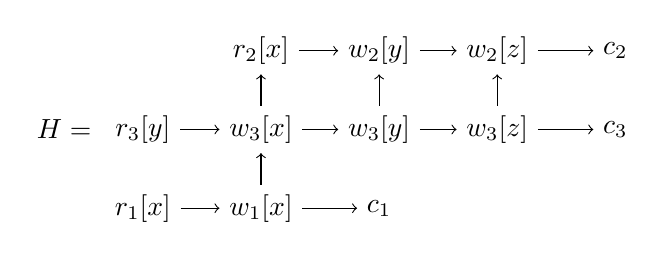
\begin{tikzpicture}
	\node (c2) at (1.5cm,2.0cm) {$r_2[x]$};
	\node (c3) at (3.0cm,2.0cm) {$w_2[y]$};
	\node (c4) at (4.5cm,2.0cm) {$w_2[z]$};
	\node (c5) at (6.0cm,2.0cm) {$c_2$};
	\node () at (-1.0cm,1.0cm) {$H=$};
	\node (b1) at (0.0cm,1.0cm) {$r_3[y]$};
	\node (b2) at (1.5cm,1.0cm) {$w_3[x]$};
	\node (b3) at (3.0cm,1.0cm) {$w_3[y]$};
	\node (b4) at (4.5cm,1.0cm) {$w_3[z]$};
	\node (b5) at (6.0cm,1.0cm) {$c_3$};
	\node (a1) at (0.0cm,0.0cm) {$r_1[x]$};
	\node (a2) at (1.5cm,0.0cm) {$w_1[x]$};
	\node (a3) at (3.0cm,0.0cm) {$c_1$};
	\path [->] (c2) edge (c3);
	\path [->] (c3) edge (c4);
	\path [->] (c4) edge (c5);
	
	\path [->] (b2) edge (c2);
	\path [->] (b3) edge (c3);
	\path [->] (b4) edge (c4);
	
	\path [->] (b1) edge (b2);
	\path [->] (b2) edge (b3);
	\path [->] (b3) edge (b4);
	\path [->] (b4) edge (b5);
	
	\path [->] (a2) edge (b2);
	
	\path [->] (a1) edge (a2);
	\path [->] (a2) edge (a3);
\end{tikzpicture}
\end{center}
\caption[Transaction History]{A history for three transactions.}
\label{fig_history}
\end{figure}

A history $H$ is \emph{serial}, if for every two transactions $T_i$ and $T_j$ in $H$, either all operations from $T_i$ appear before all operations of $T_j$ or vice versa.


% ------------------------------------------------------------------------------------------------ %
% EQUIVALENT HISTORIES
% ------------------------------------------------------------------------------------------------ %


\subsubsection{Equivalent Histories}

Two histories $H_1$ and $H_2$ are equivalent, if and only if
\begin{itemize}
\item they are over the same transactions and contain the same operations and
\item conflicting operations $p_i$ and $p_j$ of non aborted transactions are ordered in the same way in both histories, i.e $p_i <_{H_1} p_j$ holds if and only if $p_i <_{H_2} p_j$.
\end{itemize}


% ------------------------------------------------------------------------------------------------ %
% SERIALIZABLE HISTORY
% ------------------------------------------------------------------------------------------------ %


\subsubsection{Serializable History}

A history $H$ is \emph{serializable} if and only if it is equivalent to a serial history $H_s$. 

The \emph{serializability graph} $\msf{SG}(H)$ of a history $H$ over the transactions $T_1,\ldots,T_n$ is a compact representation of the dependencies in $H$. For every pair of conflicting operations $p_i$ and $q_j$ in $H$ with $p_i <_H q_j$, the edge $(T_i,T_j)$ is added to the serializability graph $\msf{SG}(H)$.

The \emph{serializability theorem} states that a history is serializable if and only if its serializability graph $\msf{SG}(H)$ is acyclic. A topological sort of $\msf{SG}(H)$ is a serial history $H_s$ with $H \equiv H_s$.

\begin{example}
	The serializability graph $\msf{SG}(H)$ of the history $H$ depicted in figure \ref{fig_history} is:
	\begin{center}
	\begin{tikzpicture}[>=latex']
		\node [draw, circle] (t2) at (1cm,1cm) {$T_2$};
		\node [draw, circle] (t1) at (0cm,0cm) {$T_1$};
		\node [draw, circle] (t3) at (2cm,0cm) {$T_3$};
		\path [->] (t1) edge (t3);
		\path [->] (t1) edge (t2);
		\path [->] (t3) edge (t2);
	\end{tikzpicture}
	\end{center}
	Thus the history $H_s = T_1 \mid T_3 \mid T_2$ is serial and equivalent to the history $H$.
\end{example}


% ------------------------------------------------------------------------------------------------ %
% RECOVERY
% ------------------------------------------------------------------------------------------------ %


\subsection{Recovery Theory}


% ------------------------------------------------------------------------------------------------ %
% RECOVERABLE HISTORIES
% ------------------------------------------------------------------------------------------------ %


\subsubsection{Recoverable Histories}

In a history $H$, a transaction $T_i$ is said to \emph{reads} from another transaction $T_j$ if
\begin{itemize}
\item $T_i$ reads a data item $x$ that was written by $T_j$, i.e there are $r_i$ and $w_j$ with $w_j[x] <_H r_i[x]$,
\item $T_j$ does not abort before the read, i.e. $a_j \not<_H r_i[x]$ and
\item if there is a write $w_k[x]$ of another transaction with $w_j[x] <_H w_k[x] <_H r_i[x]$, then there is an $a_k <_H r_i[x]$.
\end{itemize}

A history $H$ is \emph{recoverable} if for every transaction $T_i$ reads from another transaction $T_j$ the condition $c_j <_H c_i$ holds. An abort in a recoverable history does not affect already commited transactions.


% ------------------------------------------------------------------------------------------------ %
% AVOIDING CASCADING ABORTS
% ------------------------------------------------------------------------------------------------ %


\subsubsection{Avoiding Cascading Aborts}

A history $H$ \emph{avoids cascading aborts (ACA)} if all transactions $T_i$ read only from committed transactions $T_j$, i.e $c_j <_H r_i[x]$.


% ------------------------------------------------------------------------------------------------ %
% STRICT HISTORIES
% ------------------------------------------------------------------------------------------------ %


\subsubsection{Strict Histories}

A history $H$ is \emph{strict} if for all $w_j[x] <_H p_i[x]$, where $p_i$ is a read or write operation, either $a_j <_H p_i[x]$ or $c_j <_H p_i[x]$ holds.


% ------------------------------------------------------------------------------------------------ %

\begin{figure}[htb]
\begin{center}
\begin{tikzpicture}
 	\path[area, dashed] (0.0cm,0.0cm) rectangle (6.0cm,5.0cm) {};
 	\path[area] (0.2cm,0.4cm) rectangle (5.8cm,4.0cm) {};
 	\path[area] (0.4cm,0.6cm) rectangle (5.6cm,3.2cm) {};
 	\path[area] (0.6cm,0.8cm) rectangle (5.4cm,2.4cm) {};
 	\path[area] (3.2cm,1.0cm) rectangle (4.8cm,2.2cm) {};
 	\path[area] (3.0cm,0.2cm) rectangle (5.0cm,4.8cm) {};
 	\node () at (1.5cm,4.4cm) {all histories};
 	\node () at (4.0cm,4.4cm) {serializable};
 	\node () at (1.5cm,3.6cm) {recoverable};
 	\node () at (1.5cm,2.8cm) {ACA};
 	\node () at (1.5cm,2.0cm) {strict};
 	\node () at (4.0cm,1.6cm) {serial};
\end{tikzpicture}
\end{center}
\caption[Classes of Histories]{Classes of histories.}
\end{figure}


% ------------------------------------------------------------------------------------------------ %
% DATABASE SCHEDULER
% ------------------------------------------------------------------------------------------------ %


\subsection{Database Scheduler}

The task of a \emph{database scheduler} is to order the operations of transactions $T_1,\ldots,T_n$ in such a way that the resulting history is reasonable. Serializability is often the minimal requirement. In general avoidance of cascading aborts is also required.


% ------------------------------------------------------------------------------------------------ %
% LOCK BASED SYNCHRONIZATION
% ------------------------------------------------------------------------------------------------ %


\subsection{Lock Based Synchronization}

Lock based synchronization is a widely used technique for schedulers. There are two sorts of locks:
\begin{itemize}
\item A \emph{schared lock} $S$ is acquired if a transaction wants to read from an object.
\item An \emph{exclusive lock} $X$ is acquired if a transaction wants to write to an object.
\end{itemize}


% ------------------------------------------------------------------------------------------------ %
% TWO PHASE LOCKING PROTOCOL
% ------------------------------------------------------------------------------------------------ %


\subsubsection{Two-Phase Locking Protocol}

The scheduler realizes serializability by following the \emph{two-phase locking  (2PL)} protocol. The following conditions must hold:
\begin{enumerate}
\item Every transaction must acquire a lock before accessing an object.
\item A transaction acquires a lock only once. Lock upgrades are possible.
\item A transaction is blocked if the lock requested cannot be granted.
\item Every transaction goes through two phases
	\begin{enumerate}
	\item Growth: Acquire locks, but never release a lock.
	\item Schrink: Release locks, but never acquire a lock.
	\end{enumerate}
\item At the end of a transaction (commit or abort) all locks must be released.
\end{enumerate}

\begin{figure}[htbp]
\begin{center}
\begin{tikzpicture}[>=latex']
\node () at (0,1.75) {{\#}locks};
\node () at (1.8,-0.25) {growth};
\node () at (4.3,-0.25) {shrink};
\node () at (6,0) {time};
\draw [->] (0,0) -- (5.5,0);
\draw [->] (0,-0.4) -- (0,1.5);
\draw (3.6,-0.4) -- (3.6,0);
\draw [dashed] (3.6,0) -- (3.6,1.2);
\draw (5,-0.4) -- (5,0);
\draw (0,0) -- (2,1.2) -- (3.6,1.2) -- (5,0);
\end{tikzpicture}
\end{center}
\caption[Two-Phase Locking Protocol]{Visualization of the two-phase locking protocol.}
\end{figure}


% ------------------------------------------------------------------------------------------------ %
% STRICT TWO PHASE LOCKING PROTOCOL
% ------------------------------------------------------------------------------------------------ %


\subsubsection{Strict Two-Phase Locking Protocol}

The \emph{strict two-phase locking protocol} is like 2PL, except there is no shrink phase, i.e. all locks are kept until the end of the transaction.

\begin{figure}[htbp]
\begin{center}
\begin{tikzpicture}[>=latex']
\node () at (0,1.75) {{\#}locks};
\node () at (1.8,-0.25) {growth};
\node () at (5,-0.25) {EOT};
\node () at (6,0) {time};
\draw [->] (0,0) -- (5.5,0);
\draw [->] (0,0) -- (0,1.5);
\draw (0,0) -- (2,1.2) -- (5,1.2) -- (5,0);
\end{tikzpicture}
\end{center}
\caption[Strict Two-Phase Locking Protocol]{Strict two-phase locking protocol.}
\end{figure}

\begin{note}
Strict 2PL avoids cascading aborts.
\end{note}

\todo (discussion of 2PL/ S2PL)


% ------------------------------------------------------------------------------------------------ %
% DEADLOCK DETECTION
% ------------------------------------------------------------------------------------------------ %


\subsubsection{Deadlock Detection}

A precise, but expensive, way to detect \emph{deadlocks} is the \emph{wait-for graph}: For every transaction $T_i$ that waits for another transaction $T_j$, the edge $(T_i,T_j)$ is added to the graph. There is a deadlock if and only if the wait-for graph has a cycle.

\begin{example}
A wait for-graph is depicted in figure \ref{fig_waitfor}. Aborting transaction $T_2$ or $T_3$ resolves both cycles.
\end{example}

\begin{figure}[htbp]
\begin{center}
\begin{tikzpicture}[>=latex']
	\node [draw, circle] (n1) at (0,1.5) {$T_1$};
	\node [draw, circle] (n2) at (1.5,1.5) {$T_2$};
	\node [draw, circle] (n5) at (3,0.75) {$T_5$};
	\node [draw, circle] (n4) at (0,0) {$T_4$};
	\node [draw, circle] (n3) at (1.5,0) {$T_3$};
	\path [->] (n1) edge (n2);
	\path [->] (n2) edge (n3);
	\path [->] (n3) edge (n4);
	\path [->] (n4) edge (n1);
	\path [->] (n2) edge (n5);
	\path [->] (n5) edge (n3);
\end{tikzpicture}
\end{center}
\caption[Wait-For Graph]{Wait-for graph with two cycles.}
\label{fig_waitfor}
\end{figure}

Another way to detect deadlocks is to set a \emph{timeout} for every transaction's progress. If a timeout occurs, the system assumes a deadlock and resets the affected transaction.

A too short timeout leads to transactions being unnecessarily resetted, whereas a long timeout leads to prolonged deadlock situations.


% ------------------------------------------------------------------------------------------------ %
% SNAPSHOT ISOLATION
% ------------------------------------------------------------------------------------------------ %


\subsection{Snapshot Isolation}

In transaction processing, \emph{snapshot isolation (SI)} is a guarantee that all reads made in a transaction will see a consistent snapshot of the database:
\begin{enumerate}
\item When a transaction $T_i$ starts, it receives a timestamp $\tau_i$.
\item All reads are carried out as of the database at time $\tau_i$. Historic versions of all objects are needed.
\item All writes are carried out in a separate buffer and become visible after a commit.
\item When a transaction $T_i$ with timestamp $\tau_i$ commits, the DBMS checks for conflicts and aborts $T_i$ if there is another transaction $T_j$ with timestamp $\tau_j$ that updated the same object and $\tau_i < c_j < c_i$.
\end{enumerate}


\subsubsection{Lost Updates}

Figure \ref{fig_lost_update} shows two histories that are accepted by snapshot isolation, but the update of transaction $T_2$ is lost.

\begin{figure}[htbp]
\begin{center}
\begin{tabular}{|c|c|c|}\hline
  &  $T_1$   & $T_2$    \\\hline\hline
1 &          & $b_2$    \\
2 &          & $r_2[x]$ \\
3 & $b_1$    &          \\
4 & $r_1[x]$ &          \\
5 &          & $w_2[x]$ \\
6 &          & $c_2$    \\
7 & $w_1[x]$ &          \\
8 & $c_1$    &          \\\hline
\end{tabular}
\hspace{1em}
\begin{tabular}{|c|c|c|}\hline
  &  $T_1$   & $T_2$    \\\hline\hline
1 & $b_1$    &          \\
2 & $r_1[x]$ &          \\
3 &          & $b_2$    \\
4 &          & $r_2[x]$ \\
5 &          & $w_2[x]$ \\
6 &          & $c_2$    \\
7 & $w_1[x]$ &          \\
8 & $c_1$    &          \\\hline
\end{tabular}
\end{center}
\caption[Snapshot Isolation and Lost Update]{Snapshot isolation and lost update.}
\label{fig_lost_update}
\end{figure}

\subsubsection{Write Skew Anomaly}

In a \emph{write skew} anomaly, two transactions $T_1$ and $T_2$ concurrently read an overlapping data set (e.g. $x$ and $y$), concurrently make disjoint updates (e.g. $T_1$ updates $x$ and $T_2$ updates $y$, and finally commit, neither having seen the update performed by the other. In a serializable system, such an anomaly would be impossible.


\subsubsection{Comparison with Two-Phase Locking}

The history shown in figure \ref{fig_interesting} is accepted by both 2PL and SI. 2PL supports the serialization $T_2 \ra T_3 \ra T_1$ whereas SI enforces the serialization $T_1 \ra T_2 \ra T_3$, which may lead to inconsistency.

\begin{figure}[htbp]
\begin{center}
\begin{tabular}{|c|c|c|c|}\hline
   & $T_1$    & $T_2$    & $T_3$    \\\hline\hline
1  & $b_1$    &          &          \\
2  &          & $b_2$    &          \\
3  &          & $w_2[x]$ &          \\
4  &          & $w_2[y]$ &          \\
5  &          & $c_2$    &          \\
6  & $r_1[x]$ &          &          \\
7  &          &          & $b_3$    \\
8  &          &          & $r_3[z]$ \\
9  &          &          & $r_3[y]$ \\
10 &          &          & $c_3$    \\
11 & $w_1[z]$ &          &          \\
12 & $c_1$    &          &          \\\hline
\end{tabular}
\end{center}
\caption[Interesting History]{Interesting history.}
\label{fig_interesting}
\end{figure}

\begin{itemize}
\item \textbf{Two-phase locking:} A lock for every read or write is needed. There is a total order of conflicting operations. Operations are not re-ordered and only serializable histories are allowed.
\item \textbf{Snapshot isolation:} No read or write of a transaction is ever blocked; blocking only happens when a transaction commits. Aborts can be implemented very efficiently. There are no deadlocks, but unnecessary rollbacks. Non-serializable histories are allowed. Read-write conflicting operations are re-ordered and an abort is needed to deal with write-write conflicts.
\end{itemize}


% ------------------------------------------------------------------------------------------------ %
% DISTRIBUTED TRANSACTION PROCESSING
% ------------------------------------------------------------------------------------------------ %


\subsection{Distributed Transaction Processing}


% ------------------------------------------------------------------------------------------------ %
% ATOMIC COMMIT
% ------------------------------------------------------------------------------------------------ %


\subsubsection{Atomic Commit}

An \emph{atomic commit} enforces the following properties:
\begin{enumerate}
\item All processes that reach a decision reach the same one.
\item A process cannot reverse its decision.
\item A commit can only be decided if all processes vote yes.
\item If there are no failures and all processes voted yes, the decision will be to commit.
\item Consider an execution with normal failures. If all failures are repaired and no more failures occur for a sufficiently long time, then all processors will eventually reach a decision.
\end{enumerate}


% ------------------------------------------------------------------------------------------------ %
% TWO-PHASE COMMIT
% ------------------------------------------------------------------------------------------------ %


\subsubsection{Two-Phase Commit Protocol}

The \emph{two-phase commit protocol (2PC)} is a distributed algorithm that coordinates the processes that participate in a distributed atomic transaction on whether to commit or abort the transaction.

\begin{figure}[htbp]
\begin{center}
\begin{tikzpicture}[auto,>=latex',scale=\fsmscale]
	\fsmstate{s1}{0.0cm,0.0cm}{send\\ vote\\ request}
	\fsmstate{s2}{2.5cm,0.0cm}{wait for\\ votes}
	\fsmstate{s3}{4.5cm,2.0cm}{send\\ commit}
	\fsmstate{s4}{7.0cm,2.0cm}{commit}
	\fsmstate{s5}{4.5cm,-2.0cm}{send\\ abort}
	\fsmstate{s6}{7.0cm,-2.0cm}{abort}
	\draw [->] (s1) -- (s2);
	\draw [->] (s2) -- node [swap,scale=\fsmscale] {all vote yes} (s3);
	\draw [->] (s3) -- (s4);
	\draw [->] (s2) -- node [scale=\fsmscale] {some vote no} (s5);
	\draw [->] (s5) -- (s6);
\end{tikzpicture}
\end{center}
\caption[Two-Phase Commit Coordinator]{Two-phase commit coordinator.}
\label{fig_2pc_coordinator}
\end{figure}

\begin{figure}[htbp]
\begin{center}
\begin{tikzpicture}[auto,>=latex',scale=\fsmscale]
	\fsmstate{s1}{0cm,0.0cm}{wait\\ for vote\\ request}
	\fsmstate{s2}{2.0cm,2.0cm}{wait for\\ decision}
	\fsmstate{s3}{5.2cm,2.0cm}{commit}
	\fsmstate{s4}{2.0cm,-2.0cm}{abort}
	\draw [->] (s1) -- node [scale=\fsmscale] {vote yes} (s2);
	\draw [->] (s2) -- node [swap,scale=\fsmscale] {\begin{tabular}{l}commit\\[-.4em] received\end{tabular}} (s3);
	\draw [->] (s1) -- node [swap,scale=\fsmscale] {vote no} (s4);
	\draw [->] (s2) -- node [scale=\fsmscale] {\begin{tabular}{l}abort\\[-.4em] received\end{tabular}} (s4);
\end{tikzpicture}
\end{center}
\caption[Two-Phase Commit Participant]{Two-phase commit participant.}
\label{fig_2pc_participant}
\end{figure}

\begin{enumerate}
\item The coordinator sends a \textit{vote request} to all participants.
\item Upon receiving a \textit{vote request}, a participant sends a message with yes or no. If the vote is no, the participant aborts the transaction and stops.
\item If the coordinator collects all votes and
	\begin{enumerate}
	\item sends \textit{commit} if all participants voted yes or
	\item sends \textit{abort} if there is a participant that voted no.
	\end{enumerate}
\item A participant that receives a \textit{commit} or \textit{receive} from the coordinator decides accordingly and stops.7
\end{enumerate}

If the coordinator times-out waiting fo votes, it can decide to abort. If a participant times-out waiting for a \textit{vote request}, it can decide to abort. But if a participant times-out waiting for a decision it cannot decide anything; this state is called uncertainty period.

When in doubt, ask if any process has decided yet. If the coordinator fails after receiving all votes but before sending any \textit{commit} message, all participants are uncertain and will not be able to decide anything until the coordinator recovers; they are blocked.

\begin{note}
2PC meets the five atomic commit conditions.
\end{note}


% ------------------------------------------------------------------------------------------------ %
% LINEAR TWO-PHASE COMMIT
% ------------------------------------------------------------------------------------------------ %


\subsubsection{Linear Two-Phase Commit Protocol}

The \emph{linear two-phase commit protocol} exploits a linear network topology to minimize the number of messages. The process $P_1$ starts the voting phase. If a process $P_i$ receives a \textit{yes} and wants to commit, it sends a \textit{yes} to process $P_{i+1}$. If the process $P_n$ receives a \textit{yes} and wants to commit, a \textit{commit} is sent back along all processes. If any process $P_i$ receives a \textit{yes} and wants to abort, it sends an \textit{abort} to $P_{i-1}$ and $P_{i+1}$. If a process receives an abort from one side, the abort is forwarded to the other side.

\begin{figure}[htbp]
\begin{center}
\begin{tikzpicture}[auto,>=latex']
\node [draw, circle, minimum width=0.8cm] (p1) at (0.0cm,0cm) {}; \node () at (0.0cm,0cm) {$P_1$};
\node [draw, circle, minimum width=0.8cm] (p2) at (1.5cm,0cm) {}; \node () at (1.5cm,0cm) {$P_2$};
\node [draw, circle, minimum width=0.8cm] (p3) at (3.0cm,0cm) {}; \node () at (3.0cm,0cm) {$P_3$};
\node [draw, circle, minimum width=0.8cm] (p4) at (4.5cm,0cm) {}; \node () at (4.5cm,0cm) {$P_{n-1}$};
\node [draw, circle, minimum width=0.8cm] (p5) at (6.0cm,0cm) {}; \node () at (6.00cm,0cm) {$P_n$};

\path [->] (p1) edge [bend left=] node [scale=\fsmscale] {\begin{tabular}{c}yes, \\[-.4em]abort\end{tabular}} (p2);
\path [->] (p2) edge [bend left] node [scale=\fsmscale] {\begin{tabular}{c}yes, \\[-.4em]abort\end{tabular}} (p3);
\path [->] (p4) edge [bend left] node [scale=\fsmscale] {\begin{tabular}{c}yes, \\[-.4em]abort\end{tabular}} (p5);
\path [<-] (p1) edge [bend right] node [scale=\fsmscale,swap] {\begin{tabular}{c}commit, \\[-.4em]abort\end{tabular}} (p2);
\path [<-] (p2) edge [bend right] node [scale=\fsmscale,swap] {\begin{tabular}{c}commit, \\[-.4em]abort\end{tabular}} (p3);
\path [<-] (p4) edge [bend right] node [scale=\fsmscale,swap] {\begin{tabular}{c}commit, \\[-.4em]abort\end{tabular}} (p5);
\path [->,dashed] (p3) edge [bend left] (p4);
\path [<-,dashed] (p3) edge [bend right] (p4);
\end{tikzpicture}
\end{center}
\caption[Linear Two-Phase Commit Protocol] {Message flow of the linear two-phase commit protocol.}
\label{fig_linear2pc}
\end{figure}

The total number of messages sent by linear 2PC is at most $2n$ instead of $3n$. But the number of rounds is $2n$ instead of only $3$.


% ------------------------------------------------------------------------------------------------ %
% THREE PHASE COMMIT
% ------------------------------------------------------------------------------------------------ %


\subsubsection{Three-Way Commit Protocol}

In the two-phase commit protocol there is the blocking situation in which all processes have voted yes but the coordinator fails. To avoid this situation the \emph{three-phase commit protocol (3PC)} enforces the non-blocking rule: \textit{No process can decide to commit if there are processes that are uncertain}.

\todo (WTF is this shit?)

\begin{figure}[htbp]
\begin{center}
\begin{tikzpicture}[auto,>=latex',scale=\fsmscale]
	\fsmstate{s1}{0.0cm,3.0cm}{send \\vote \\request}
	\fsmstate{s2}{2.5cm,3.0cm}{wait for \\votes}
	\fsmstate{s3}{5.7cm,3.0cm}{send\\ abort}
	\fsmstate{s4}{8.2cm,3.0cm}{abort}
	\fsmstate{s5}{0.0cm,0.0cm}{send\\ precommit}
	\fsmstate{s6}{2.5cm,0.0cm}{wait for\\ ACKs}
	\fsmstate{s7}{5.7cm,0.0cm}{send\\ commit}
	\fsmstate{s8}{8.2cm,0.0cm}{commit}
	\draw [->] (s1) -- (s2);
	\draw [->] (s2) -- node [swap, scale=\fsmscale] {\begin{tabular}{c}some\\[-.4em] vote no\end{tabular}} (s3);
	\draw [->] (s3) -- (s4);
	\draw [->] (s2) -- node [swap, pos=0.7, scale=\fsmscale] {all vote yes} (s5);
	\draw [->] (s5) -- (s6);
	\draw [->] (s6) -- node [scale=\fsmscale] {\begin{tabular}{c}all ACKs\\[-.4em] received\end{tabular}} (s7);
	\draw [->] (s7) -- (s8);
\end{tikzpicture}
\end{center}
\caption[Three-Way Commit Coordinator]{Three-way commit coordinator.}
\end{figure}

\begin{figure}[htbp]
\begin{center}
\begin{tikzpicture}[auto,>=latex',scale=\fsmscale]
	\fsmstate{s1}{0.0cm,3.0cm}{wait\\ for vote\\ request}
	\fsmstate{s2}{5.7cm,3.0cm}{abort}
	\fsmstate{s3}{0.0cm,0.0cm}{wait for\\ precommit}
	\fsmstate{s4}{3.2cm,0.0cm}{send\\ ACK}
	\fsmstate{s5}{5.7cm,0.0cm}{wait for\\ commit}
	\fsmstate{s6}{8.9cm,0.0cm}{commit}
	\draw [->] (s1) -- node [swap, scale=\fsmscale] {vote no} (s2);
	\draw [->] (s1) -- node [scale=\fsmscale] {vote yes} (s3);
	\draw [->] (s3) -- node [scale=\fsmscale] {\begin{tabular}{c}precommit\\[-.4em] received\end{tabular}} (s4);
	\draw [->] (s4) -- node [sloped, pos=0.9, scale=\fsmscale] {\begin{tabular}{c}abort\\[-.4em] received\end{tabular}} (s2);
	\draw [->] (s4) -- (s5);
	\draw [->] (s5) -- node [scale=\fsmscale] {\begin{tabular}{c}commit\\[-.4em] received\end{tabular}} (s6);
\end{tikzpicture}
\end{center}
\caption[Three-Way Commit Participant]{Three-way commit participant.\footnotemark}
\end{figure}

\footnotetext{This state diagram was copied from the lecture slides; but I cannot explain the transition from \textit{send ACK} to \textit{abort}.}


% ------------------------------------------------------------------------------------------------ %